\documentclass{article}

\usepackage{graphicx}
\usepackage{tikz}
\usepackage{tikzsymbols}
\usetikzlibrary{calc,patterns,shapes.geometric}
\pagestyle{empty}
\usepackage[margin=0pt]{geometry}
\geometry{papersize={14in,12in}}

\def\centerarc[#1](#2)(#3:#4:#5){\draw[#1] ($(#2)+({#5*cos(#3)},{#5*sin(#3)})$) arc (#3:#4:#5);}

\begin{document}
	\begin{figure}
		\centering
		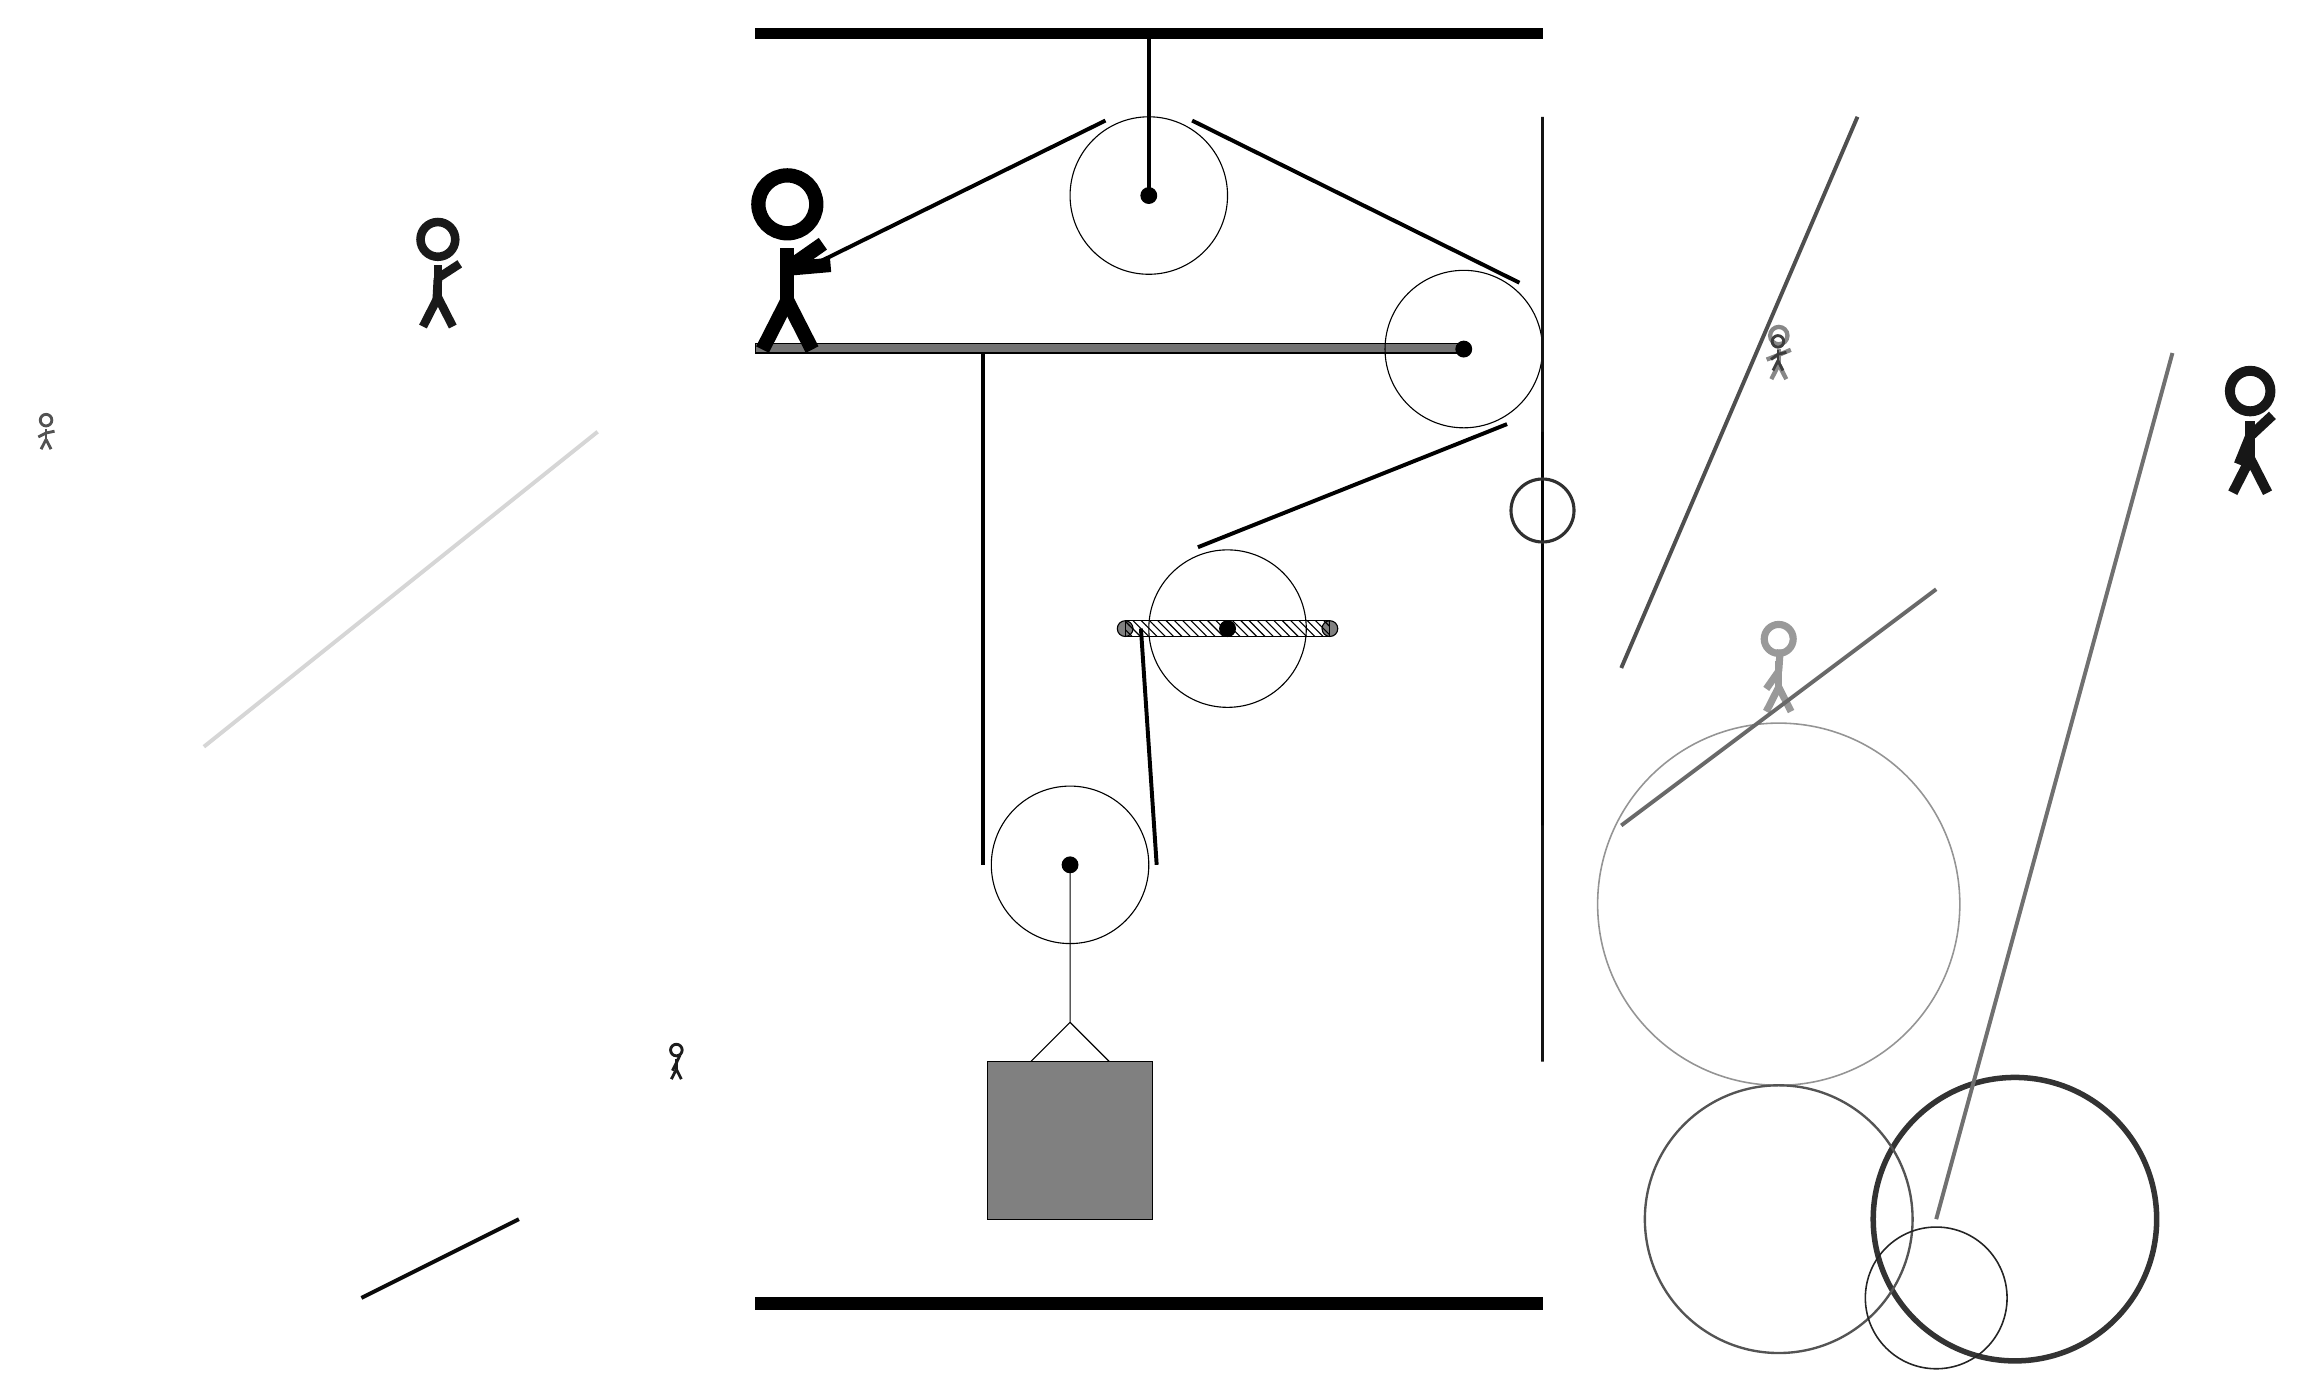
\begin{tikzpicture}
			%%%%% START %%%%%
			
			\draw[fill=black] (-2, 14) rectangle (8, 14.125);
			
			\draw[fill=black!55] (-2, 10) rectangle (7, 10.125);
			
			\draw (2, 3.5) circle (1);
			\draw[fill=black] (2, 3.5) circle (0.1);
			
			\draw (7, 10.05) circle (1);
			\draw[fill=black] (7, 10.05) circle (0.1);
			
			\draw[fill=white](4, 6.5) circle (1);
			\draw[fill=black] (4, 6.5) circle (0.1);
			\draw[fill=black!50] (2.7, 6.5) circle (0.1);
			\draw[fill=black!50] (5.3, 6.5) circle (0.1);
			\draw[pattern=north west lines, pattern color=black] (2.7, 6.6) rectangle (5.3, 6.4);
			
			\draw (3, 12) circle (1);
			\draw[fill=black] (3, 12) circle (0.1);
			\draw[line width=0.5mm] (3, 12) -- (3, 14);
			
			\draw (2, 3.5) -- (2, 1.5) -- (1.5, 1.0) -- (2.5, 1.0) -- (2, 1.5);
			\draw[fill=black!50] (0.95, 1.0) rectangle (3.05, -1.0);
			
			\draw[line width=0.5mm] (0.9, 10) -- (0.9, 3.5);
			\centerarc[line width=0.5mm](2, 3.5)(180:360:1.1);
			\draw[line width=0.5mm](3.1, 3.5) -- (2.9, 6.5);
			\centerarc[line width=0.5mm](4, 6.5)(110:180:1.1);
			\draw[line width=0.5mm](3.6238, 7.5337) -- (7.55, 9.0974);
			\centerarc[line width=0.5mm](7, 10.05)(-60:50:1.1);
			\draw[line width=0.5mm](7.7071, 10.8926) -- (3.55, 12.9526);
			\centerarc[line width=0.5mm](3, 12)(60:120:1.1);
			\draw[line width=0.5mm](2.45, 12.9526) -- (-1.2, 11.15);
			
			\node[line width=0.4mm, color=black!47] at (11, 10) {\Strichmaxerl[3][21][23]};
			
			\draw [line width=0.2mm, color=black!42](11, 3) circle (2.3);
			\draw [line width=0.7mm, color=black!80](14, -1) circle (1.8);
			\draw [line width=0.3mm, color=black!67](11, -1) circle (1.7);
			\draw[line width=0.5mm, color=black!69](12, 13) -- (9, 6);
			
			\draw[line width=0.5mm, color=black!56](13, -1) -- (16, 10);
			\draw [line width=0.2mm, color=black!86](13, -2) circle (0.9);
			\draw[line width=0.5mm, color=black!16](-4, 9) -- (-9, 5);
			\draw[line width=0.3mm, color=black!92] (8, 1) rectangle (8, 13);
			
			\node[line width=0.5mm, color=black!40] at (11, 6) {\Strichmaxerl[5][55][86]};
			
			\node[line width=0.7mm, color=black!76] at (11, 10) {\Strichmaxerl[2][37][13]};
			\draw[line width=0.5mm, color=black!59](13, 7) -- (9, 4);
			\node[line width=0.6mm, color=black!90] at (-6, 11) {\Strichmaxerl[6][87][33]};
			
			\draw[line width=0.3mm, color=black!98] (8, 4) rectangle (8, 9);
			\node[line width=0.6mm, color=black!89] at (-3, 1) {\Strichmaxerl[2][63][65]};
			\node[line width=0.6mm, color=black!91] at (17, 9) {\Strichmaxerl[7][68][43]};
			
			\draw [line width=0.4mm, color=black!81](8, 8) circle (0.4);
			\node[line width=0.4mm, color=black!68] at (-11, 9) {\Strichmaxerl[2][27][12]};
			\draw[line width=0.5mm, color=black!96](-7, -2) -- (-5, -1);
			
			\node at (-1.5, 11.15) {\Strichmaxerl[10][-175][35]};
			
			\draw[fill=black] (-2, -2) rectangle (8, -2.15);
			
			%%%%% END %%%%%
		\end{tikzpicture}
	\end{figure}	
\end{document}